
% This LaTeX was auto-generated from an M-file by MATLAB.
% To make changes, update the M-file and republish this document.

\documentclass{article}
\usepackage{graphicx}
\usepackage{color}

\sloppy
\definecolor{lightgray}{gray}{0.5}
\setlength{\parindent}{0pt}

\begin{document}

    
    
\subsection*{Contents}

\begin{itemize}
\setlength{\itemsep}{-1ex}
   \item Ejercicio 1 - Introducción y repaso de probabilidad y teoría de información
   \item Ejercicio 1.1
   \item 1.i) $fdp$ gaussiana unidimensional
   \item randgauss.m
   \item randgauss1D.m
   \item 1.ii y 1.iii) $fdp$ gaussiana bidimensional [no] correlacionada;
   \item mvrandgauss.m
   \item randgaussXD.m
   \item Ejercicio 1.2
   \item Ejercicio 1.3
\end{itemize}


\subsection*{Ejercicio 1 - Introducción y repaso de probabilidad y teoría de información}

\begin{par}
Escriba un programa para generar números aleatorios $\mathbf{x}$ con una función de densidad de probabilidad ($fdp$) gaussiana $\mathcal{N}(\mathbf{\mu},\mathbf{\Sigma})) en $d$ dimensiones.
\end{par} \vspace{1em}
\begin{verbatim}
clc; close all; clear all;
\end{verbatim}


\subsection*{Ejercicio 1.1}

\begin{par}
Para cada uno de los siguientes casos: i) $fdp$ gaussiana unidimensional, ii) $fdp$ gaussiana bidimensional no correlacionada y iii) $fdp$ gaussiana bidimensional correlacionada,
\end{par} \vspace{1em}
\begin{itemize}
\setlength{\itemsep}{-1ex}
   \item Genere un conjunto de números aleatorios con esa $fdp$.
   \item Estime la $fdp$ experimental mediante un histrograma normalizado.
   \item Compare gráficamente la estimación obtenida con la fdp teórica.
\end{itemize}


\subsection*{1.i) $fdp$ gaussiana unidimensional}

\begin{verbatim}
N      = 5000;  %
media  = 3;     % definición de la fdp
desvio = 2;     %

x = randgauss1D(media, desvio, N);  % conjunto de números aleatorios

[alturas, centros] = hist(x, 40);   % histograma sin normalizar
ancho = centros(2) - centros(1);    % ancho de las barras del histograma
area  = sum(ancho .* alturas);      % area de las barras del histograma
fdpexp = alturas/area;              % fdp experimental
bar(centros, fdpexp,'w');           % dibuja histograma normalizado

% Comparación con la fdp teórica
t = -7:0.01:13;
fdpteor = normpdf(t,media,desvio); % fdp teórica con igual media y desvio
hold on; plot(t,fdpteor,'-k','LineWidth',2); hold off;

title({'fdp de una distribucion gaussiana unidimensional';
       sprintf('mu = %0.1f, sigma = %0.1f', media, desvio)})
ylabel('p(x)'); xlabel('x');
legend('fdp experimental','fdp teorica')
\end{verbatim}

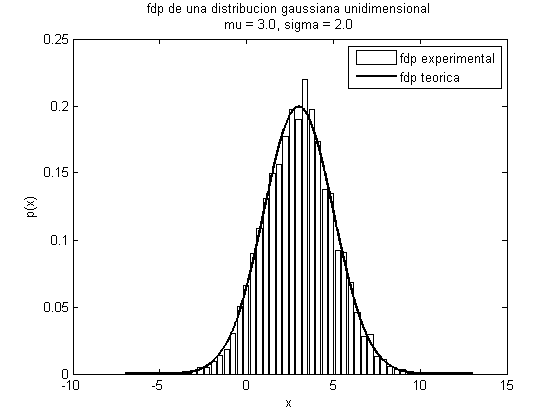
\includegraphics [width=4in]{Ejercicio1_01.png}
\begin{par}
Para normalizar el histograma se dividió por la suma de las áreas de los rectángulos dado que la integral de una $fdp$ debe dar 1, aún en este caso donde la $fdp$ es empírica. En la comparación gráfica se verifica la correspondencia con la $fdp$ teórica.
\end{par} \vspace{1em}
\begin{par}
Debajo se muestra el código de las dos funciones utilizadas para generar números aleatorios de una distribución normal unidimensional.
\end{par} \vspace{1em}


\subsection*{randgauss.m}

\begin{verbatim}
dbtype randgauss.m
\end{verbatim}

        \color{lightgray} \begin{verbatim}
1     function x = randgauss()
2     %RANDGAUSS() genera un número pseudo aleatorio de una distribución 
3     % gaussiana estándar. 
4     %  El número x es generado por el método polar de Box-Muller a partir de 
5     %  dos números pseudo aleatorios independentes y uniformemente 
6     %  distribuidos en un intervalo cerrado [−1, +1]
7     %  Referencias: 
8     %  - Box, G. E. P. and Muller, M. E. "A Note on the Generation of Random 
9     %    Normal Deviates." Ann. Math. Stat. 29, 610-611, 1958.
10    %  - Bell, J.,  "Algorithm 334: Normal random deviates", Communications 
11    %    of the ACM, vol. 11, No. 7. 1968
12    
13    s=1; % condición para ingresar al while
14    while (s >= 1) || (s == 0)
15        % u1 y u2 independientes y distribuidos uniformemente en [-1, +1]
16        u1 = 2.0 * rand() - 1.0;
17        u2 = 2.0 * rand() - 1.0;
18    	
19        s = u1 .* u1 + u2 .* u2; % variable a evaluar
20    end
21    % a la salida s está uniformemente distribuido en (0, +1)
22    
23    % número aleatorio de una distribución normal estándar
24    x = u1 .* sqrt( (-2.0 .* log( s ) ) ./ s ); 
25    
26    end
27    

\end{verbatim} \color{black}
    

\subsection*{randgauss1D.m}

\begin{verbatim}
dbtype randgauss1D.m
\end{verbatim}

        \color{lightgray} \begin{verbatim}
1     function x = randgauss1D(mu, sigma, N)
2     %RANDGAUSS1D(mu, sigma, N) genera un vector de números aleatorios con 
3     %distribución gaussiana de media mu y desvío sigma. Los valores por defecto
4     %son mu = 0, sigma = 1 y N = 1. El vector x es vertical (de tamaño N x 1).
5     
6     if nargin < 1
7         mu = 0;    % media por defecto
8     end
9     if nargin < 2
10        sigma = 1; % desvío por defecto
11    end
12    if nargin < 3
13        N = 1;     % tamaño por defecto
14    end
15    
16    x = zeros(N,1); % inicializo
17    for n = 1:N
18        x(n) = randgauss(); % relleno el vector
19    end
20    x = mu + sigma .* x; % ajusto a mu y sigma
21    
22    end
23    

\end{verbatim} \color{black}
    

\subsection*{1.ii y 1.iii) $fdp$ gaussiana bidimensional [no] correlacionada;}

\begin{verbatim}
meds{1} = [50 100]; %
covs{1} = [2 0;     % definición de fdp no correlacionada
           0 1];    %
titulos{1} = ['fdp de una distribucion gaussiana bidimensional no ' ...
              'correlacionada'];

meds{2} = [50 100]; %
covs{2} = [2 1;     % definición de fdp correlacionada
           1 1];    %
titulos{2} = ['fdp de una distribucion gaussiana bidimensional ' ...
              'correlacionada'];

% Realizo la misma comparacion para los casos ii) y iii)
for k = 1:2
media = meds{k};
covar = covs{k};
titulo = titulos{k};
figure('units','normalized','outerposition',[0 0 1 1]);
suptitle({titulo; sprintf(['mu = [%0.0f %0.0f], '...
                           'sigma = [%0.0f %0.0f; %0.0f %0.0f]'],...
                          media, covar)})

N = 10000;                         % cantidad de muestras
x = randgaussXD(media, covar, N);  % conjunto de números aleatorios

[alturas, centros] = hist3(x,[15 15]);          % histograma sin normalizar
ancho1 = centros{1}(2) - centros{1}(1);         % ancho de las barras en x1
ancho2 = centros{2}(2) - centros{2}(1);         % ancho de las barras en x2
volumen = sum(ancho1 * sum(ancho2 * alturas));  % volumen de las barras
fdpexp = alturas ./ volumen;                    % fdp experimental

subplot(1,2,1);                      % grafica de la malla y teorica en 3D
mesh(centros{1},centros{2},fdpexp'); % mesh necesita la matriz traspuesta

% Contour plot de la fdp experimental
% hold on; contour3(centros{1},centros{2},0.01+fdpexp','k-'); hold off

% comparacion con la fdp teorica
NN = 100;
t1 = linspace(44,56,NN); t2 = linspace(96,104,NN);
fdpteor = zeros(NN);
for i = 1:NN
    for j = 1:NN
        fdpteor(i,j) = mvnpdf([t1(i) t2(j)],media,covar);
    end
end
hold on; contour3(t1,t2,0.005+fdpteor','k-'); hold off
axis tight;
daspect([max(daspect)*[1 1] 2]);% relacion de aspecto en x1 y x2

ylabel('x_2'); xlabel('x_1'); zlabel('p(x_1,x_2)');
legend('fdp experimental','fdp teorica', 'Location','West')
title('Superficie de nivel')

% curvas de nivel de la teorica y la experimental
subplot(1,2,2);
% contour necesita la matriz traspuesta
contour(centros{1},centros{2},fdpexp',5,'k');          % fdp experimental
hold on; contour(t1,t2,0.01+fdpteor',5,'b:'); hold off % fdp teorica
axis equal; axis([46 54 97 103]);

ylabel('x_2'); xlabel('x_1');
title('Curvas de nivel')
legend('fdp experimental','fdp teorica')

end
\end{verbatim}

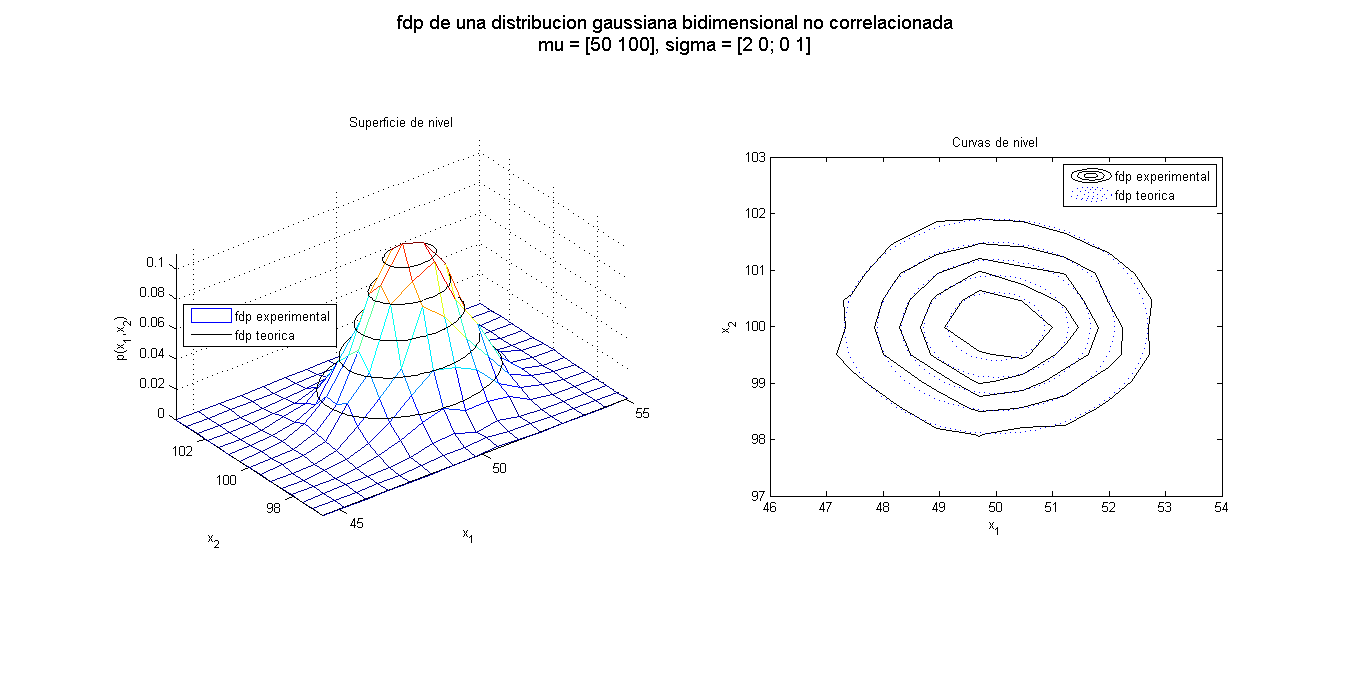
\includegraphics [width=4in]{Ejercicio1_02.png}

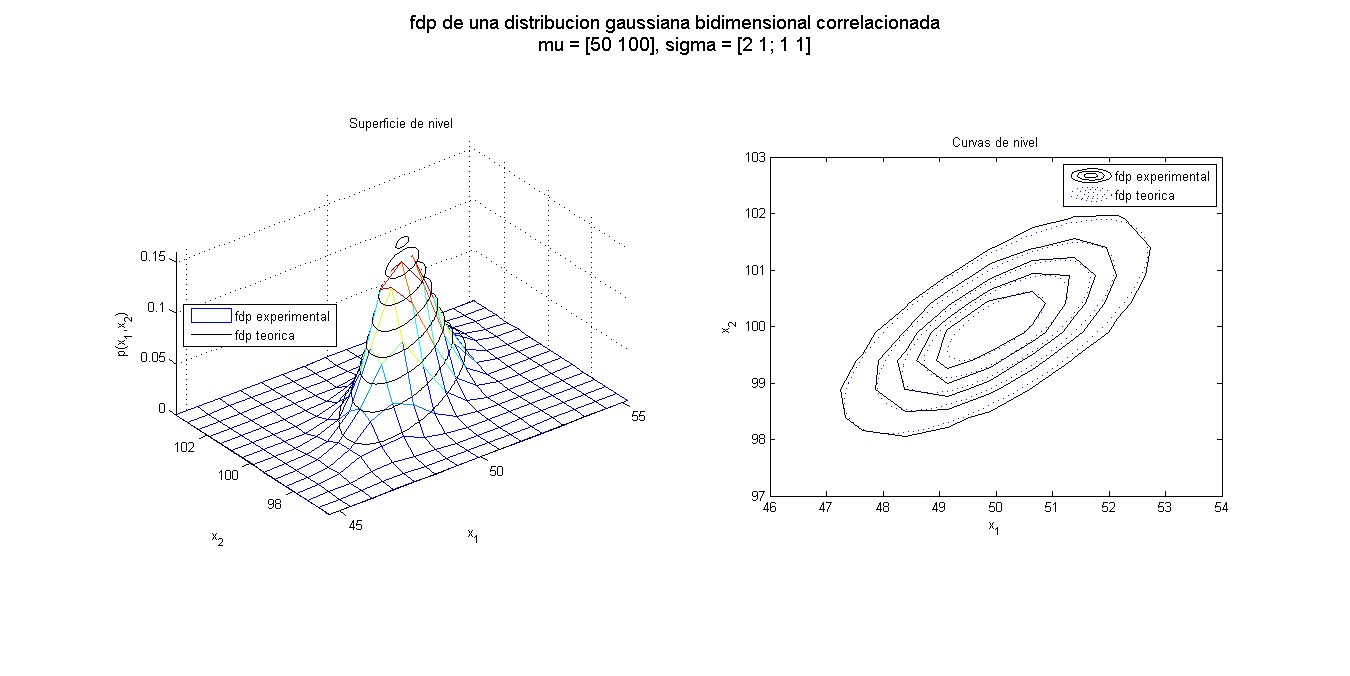
\includegraphics [width=4in]{Ejercicio1_03.png}
\begin{par}
Para normalizar el histograma se dividió por la suma total de los volúmenes de todos los prismas, análogo al caso unidimensional donde se sumaron las áreas de las barras.
\end{par} \vspace{1em}
\begin{par}
Para la comparación gráfica con la distribución teórica se utilizaron superficies y curvas de nivel. En ambos casos se comprobó el parecido entre la $pdf$ teórica y experimental.
\end{par} \vspace{1em}
\begin{par}
Debajo se muestra el código de las dos funciones utilizadas para generar los conjuntos de números de una distribución normal bidimensional. \texttt{mvrandgauss.m} utiliza \texttt{randgauss.m} como punto de partida e incluye la demostración del funcionamiento dentro de su código.
\end{par} \vspace{1em}


\subsection*{mvrandgauss.m}

\begin{verbatim}
dbtype mvrandgauss.m
\end{verbatim}

        \color{lightgray} \begin{verbatim}
1     function x = mvrandgauss(MU, SIGMA)
2     %MVRANDGAUSS genera un número aleatorio de dimensión D proveniente de una 
3     % distribución gaussiana multidimensional cuyas medias quedan definidas
4     % por el vector MU (horizontal, de tamaño D x 1) y la matriz de covarianza 
5     % SIGMA (cuadrada, de tamaño D x D)
6     % Los valores por defecto son MU = 0 y SIGMA = matriz identidad.
7     
8     if nargin < 1
9         MU = 0;
10    end
11    if nargin < 2
12        SIGMA = eye(length(MU));
13    end
14    D = size(SIGMA,1);
15    
16    if (size(MU,2) ~= D) || (size(MU,1) ~= 1) || (D ~= size(SIGMA,2))
17       error(message('Error en los tamaños de MU o SIGMA'));
18    end
19    
20    % Como SIGMA es definida positiva puede usarse la descomposición de Cholesky 
21    triangSup = chol(SIGMA); % SIGMA = triangSup' * triangSup
22    
23    % z es un número aleatorio normal estándar de tamaño 1 x D
24    z = randgauss1D(0,1,D)';  % E[z' * z] = I
25    
26    x = z * triangSup + MU;
27    
28    % Demostración de que la expresión anterior devuelve el resultado esperado
29    % -------------------------------------------------------------------------
30    % Si se toma x = z * triangSup se cumple que:
31    % E[x' * x] = E[(z * triangSup)' * (z * triangSup)]
32    %           = E[ triangSup' * z' * z * triangSup ]
33    %           = triangSup' * E[ z' * z ] * triangSup
34    %           = triangSup' * I * triangSup
35    %           = triangSup' * triangSup
36    %           = SIGMA
37    % Entonces z * triangSup cumple con la matriz de covarianza dada SIGMA
38    % Por último desplazo la distribución con MU sin alterar  E[x' * x]
39    
40    end
\end{verbatim} \color{black}
    

\subsection*{randgaussXD.m}

\begin{verbatim}
dbtype randgaussXD.m
\end{verbatim}

        \color{lightgray} \begin{verbatim}
1     function x = randgaussXD(MU, SIGMA, N)
2     %RANDGAUSSXD(MU, SIGMA, N) genera un conjunto de números aleatorios de 
3     % dimensión D provenientes de una distribución gaussiana multidimensional, 
4     % cuyas medias quedan definidas por el vector MU (horizontal, de tamaño 
5     % 1 x D), la matriz de covarianza SIGMA (cuadrada, de tamaño D x D) y la
6     % cantidad de numeros N (1 por defecto). 
7     %
8     % x es de tamaño N x D, donde cada número de dimensión D se ubica por
9     % renglón.
10    
11    if nargin < 3
12        N = 1;     % tamaño por defecto
13    end
14    
15    x = zeros(N,length(MU)); % inicializo
16    for n = 1:N
17        x(n,:) = mvrandgauss(MU, SIGMA); % Conjunto de números aleatorios
18    end
19    
20    end
21    

\end{verbatim} \color{black}
    

\subsection*{Ejercicio 1.2}

\begin{par}
Compruebe numéricamente el teorema del límite central mediante la suma de números aleatorios con distribución uniforme.
\end{par} \vspace{1em}
\begin{verbatim}
repeticiones = 10000; % veces a repetir el calculo del promedio
N = [1 2 4 40];       % numeros a promedior
promedio = zeros(1,repeticiones);
figure
for n = 1:length(N)
    for r = 1:repeticiones
        % suma de N números aleatorios en [-1, +1]
        promedio(r) = (1/N(n)) * sum(2*rand(1,N(n))-1);
    end
    subplot(2,2,n)
    hist(promedio,40)
    title(['Promedio entre ' num2str(N(n)) ' numeros'])
end
\end{verbatim}

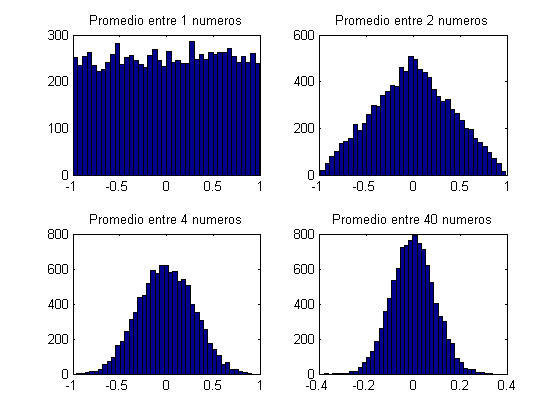
\includegraphics [width=4in]{Ejercicio1_04.png}


\subsection*{Ejercicio 1.3}

\begin{par}
Estime numéricamente y compare con el valor teorico, la entropia de una variable aleatoria con distribucion: i) laplaciana; ii) gaussiana y iii) uniforme.
\end{par} \vspace{1em}
\begin{verbatim}
N=1000;

% mantengo media y desvio para las 3 distribuciones
media = 3;
desvio = 2;

% numeros provenientes de una distribuci�n gaussiana
xgauss = media + desvio*randn(N,1);

% numeros provenientes de una distribuci�n uniforme
ini = media - sqrt(3) * desvio;
fin = media + sqrt(3) * desvio;
xunif = ini + (fin - ini) .* rand(N,1);

% numeros provenientes de una distribuci�n laplaciana
media = 5;
beta  = desvio/sqrt(2);
xlap  = randlap(N,media,beta);

% Calculo de entropias teoricas y emp�ricas
HgaussTeorica  = 0.5 * (1 + log(2*pi*desvio.^2) )
HgaussEmpirica = entropia(xgauss)

HunifTeorica  = log(fin - ini)
HunifEmpirica = entropia(xunif)

HlapTeorica  = 1 + log(2*beta)
HlapEmpirica = entropia(xlap)
\end{verbatim}

        \color{lightgray} \begin{verbatim}
HgaussTeorica =

    2.1121


HgaussEmpirica =

    2.9484


HunifTeorica =

    1.9356


HunifEmpirica =

    3.3845


HlapTeorica =

    2.0397


HlapEmpirica =

    2.3636

\end{verbatim} \color{black}
    \begin{par}
La entropia teorica de cada distribuci�n esta calculada para la versi�n cont�nua de la funci�n de densidad de probabilidad (fdp). En cambio, la entrop�a empirica es calculada por media de una aproximaci�n de la fdp. Esto ocasiona las diferencias observadas en los valores anteriores. Adem�s es sabido que la entrop�a discreta no es equivalente a la entrop�a te�rica
\end{par} \vspace{1em}



\end{document}
    
